\section{Auswertung}
\label{sec:Auswertung}

Für die Auswertung wird die \texttt{Python}-Bibliothek \texttt{numpy} \cite{numpy} benutzt. Die Fits entstehen mit \texttt{curve\_fit} aus \texttt{scipy.optimize} \cite{scipy}.
Die Fehlerrechnung wird mit \texttt{uncertainties} \cite{uncertainties} durchgeführt. Plots entstehen mit \texttt{matplotlib.pyplot} \cite{matplotlib}.

\subsection{Fehler}
Der Mittelwert $\bar{x}$ von $N$ gemessenen Werten $a$ bestimmt sich über
\begin{equation}
    \bar{x} = \frac{1}{N} \sum^N_{i=1} a_i,
    \label{eq:mittelwerte}
\end{equation}
der Fehler des Mittelwertes über
\begin{equation}
    \Delta x = \sqrt{\frac{1}{N \cdot (N-1)} \sum^N_{i=1}(a_i - \bar{x})}.
    \label{eq:mittelwerte_fehler}
\end{equation}
Die Gaußsche Fehlerfortpflanzung für eine berechnete Größe $f$ lautet
\begin{equation}
    \Delta f = \sqrt{ \sum^N_{i=1} \left( \frac{\delta f}{\delta x_i}\right)^2 \cdot (\Delta x_i)^2}.
\end{equation}
Prozentuale Abweichungen werden mit
\begin{equation}
    \Delta x = \left|\frac{x - a}{a}\right|
    \label{eq:abweichung}
\end{equation}
berechnet, wobei $a$ ein Vergleichswert und $x$ der erhaltene Wert ist.

\subsection{Heizraten}
Zur Bestimmung der Heizraten wurden die Temperaturen gegen die Zeit aufgetragen. Dazu wurden die
Einheit von $°C$ in $K$ umgerechnet. Aus den Daten wurde eine lineare Funktion der Form 
\begin{equation}
    I(t)= a_it+b_i 
\end{equation}
gebildet um die Heizraten zu ermitteln. Der Einfachheit halber ist bei den Strömen eine Unsicherheit
von $0.05\cdot10^{-11}$ \(A\)angenommen worden, obwohl dieser kleiner sein könnte.
Für die Temperatur wurde ein Fehler von 0.3 K angenommen.

\begin{figure}[H]
    \centering
    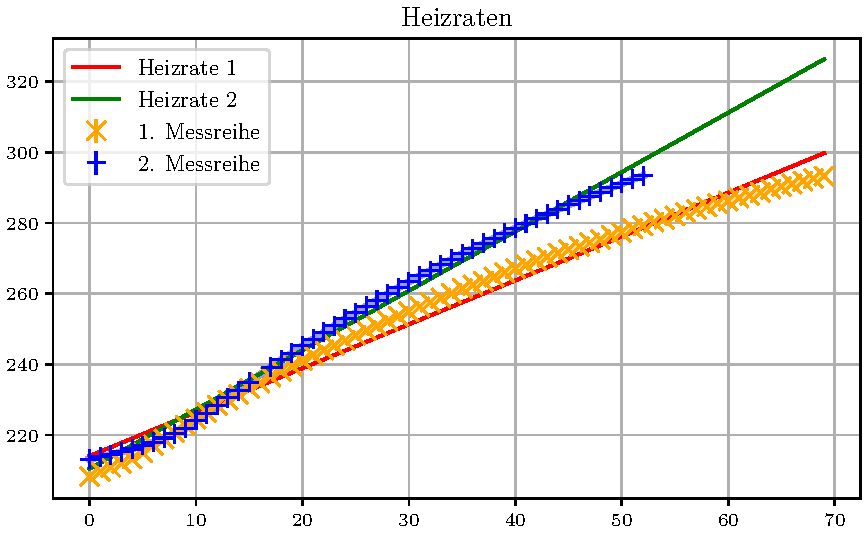
\includegraphics[width=\textwidth]{plots/A_heizraten.pdf}
    \caption{Die Heizraten für beide Messreihen}
    \label{fig:Heizraten}
\end{figure}

Die Heizraten für die beidem Messreihen ergeben sich zu:
\begin{equation}
b_1 =  \qty{1.24(1)}{\kelvin\per\minute}
\end{equation}
\begin{equation}
b_2 = \qty{1.67(2)}{\kelvin\per\minute}
\end{equation}

\subsection{Hintergrundsignale und Datenbereinigung}
In den Abbildungen \ref{fig:Hintergrund1} und \ref{fig:Hintergrund2} werden die Messdaten grafisch dargestellt.
Für die Analyse wird ein linearer Hintergrund angenommen, der mithilfe der ausgleichsgeraden berechnet wird.

\begin{figure}[H]
    \centering
    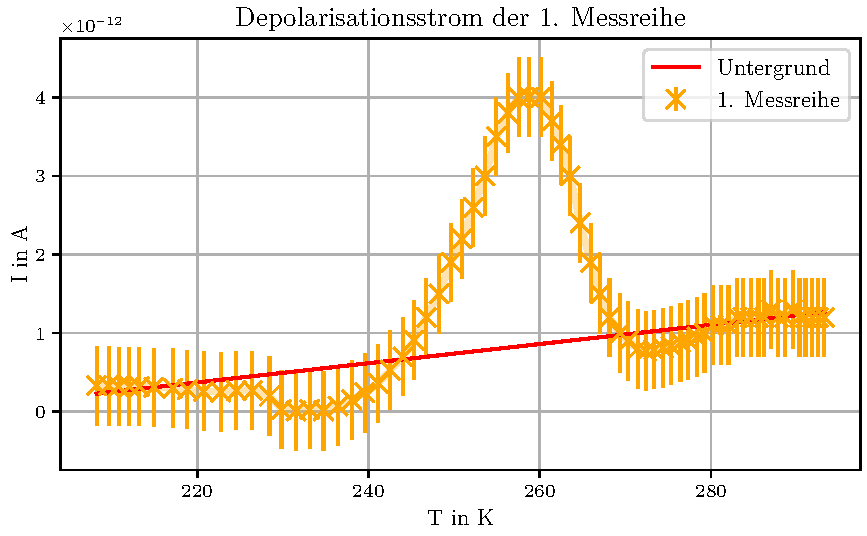
\includegraphics[width=\textwidth]{plots/B_messreihe1.pdf}
    \caption{Der erste Datensatz zusammen mit der linearen Regression des Hintergrundes für die erste Messreihe.}
    \label{fig:Hintergrund1}
\end{figure}

\begin{figure}[H]
    \centering
    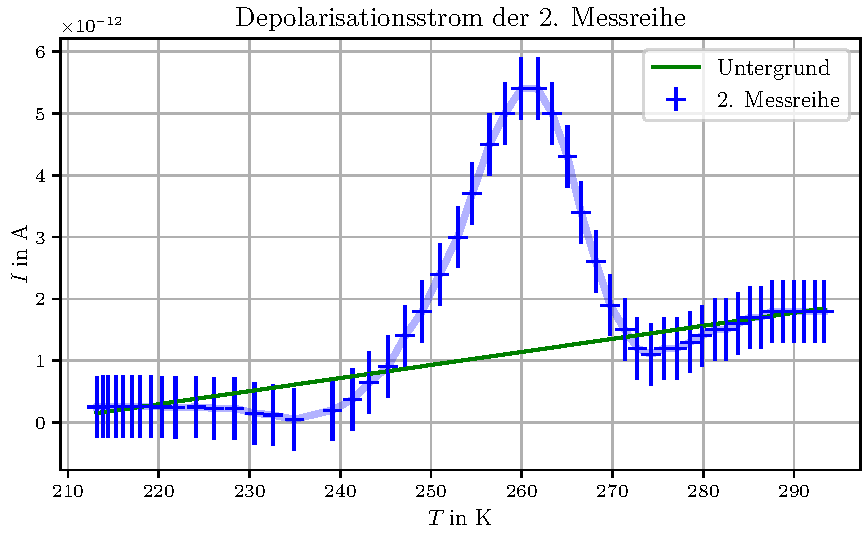
\includegraphics[width=\textwidth]{plots/C_messreihe2.pdf}
    \caption{Der zweite Datensatz zusammen mit der linearen Regression des Hintergrundes für die zweite Messreihe.}
    \label{fig:Hintergrund2}
\end{figure}

Die Paramneter der Ausgleichsfunktion lauten:
\begin{equation}
f(t) = \qty{0.0122(4)}{\ampere\per\kelvin} \cdot T - \qty{2.315(98)}{\ampere}
\end{equation}
\begin{equation}
f(t) = \qty{0.0211(5)}{\ampere\per\kelvin} \cdot T - \qty{4.356(121)}{\ampere}
\end{equation}
Diese lineare Funktion wird verwendet, um den Einfluss des Hintergrundes auf die Messreihe zu beschreiben und zu korrigieren,
sodass nur die relevanten Effekte des Depolarisationsstroms analysiert werden. Um die Messdaten von dem 
Hintergrund zu bereinigen wird er von den Daten subtrahiert.

Die bereinigten Messwerte sind in \ref{fig:Bereinigt1} und \ref{fig:Bereinigt2}  zu sehen.

\begin{figure}[H]
    \centering
    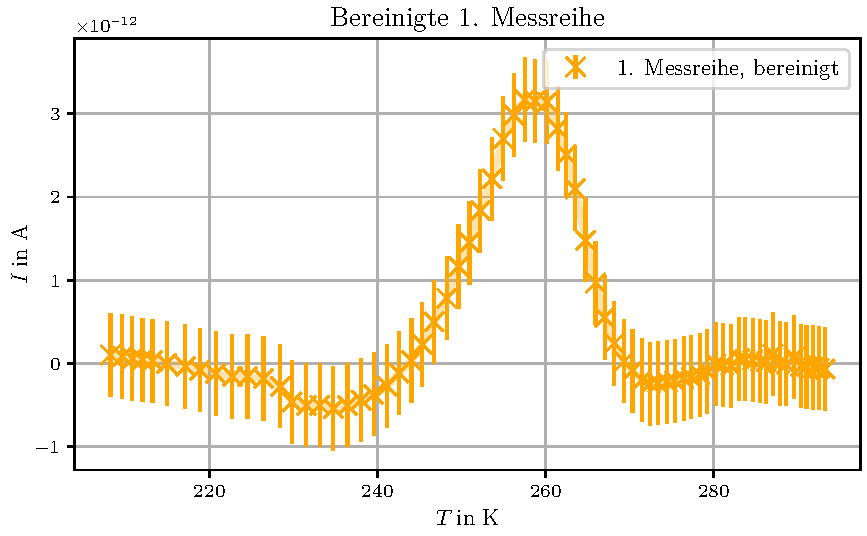
\includegraphics[width=\textwidth]{plots/D_messreihe1_bereinigt.pdf}
    \caption{Die bereinigte erste Messreihe.}
    \label{fig:Bereinigt1}
\end{figure}

\begin{figure}[H]
    \centering
    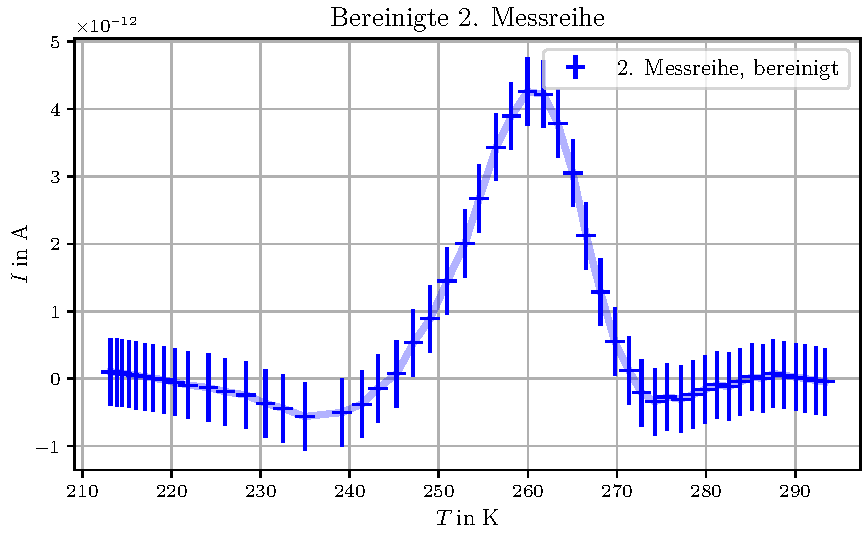
\includegraphics[width=\textwidth]{plots/E_messreihe2_bereinigt.pdf}
    \caption{Die bereinigte zweite Messreihe.}
    \label{fig:Bereinigt2}
\end{figure}

Für die Fits sind insbesondere die gaußähnlichen Datenpunkte relevant in \ref{fig:Vergleich} sind diese dargestellt.

\begin{figure}[H]
    \centering
    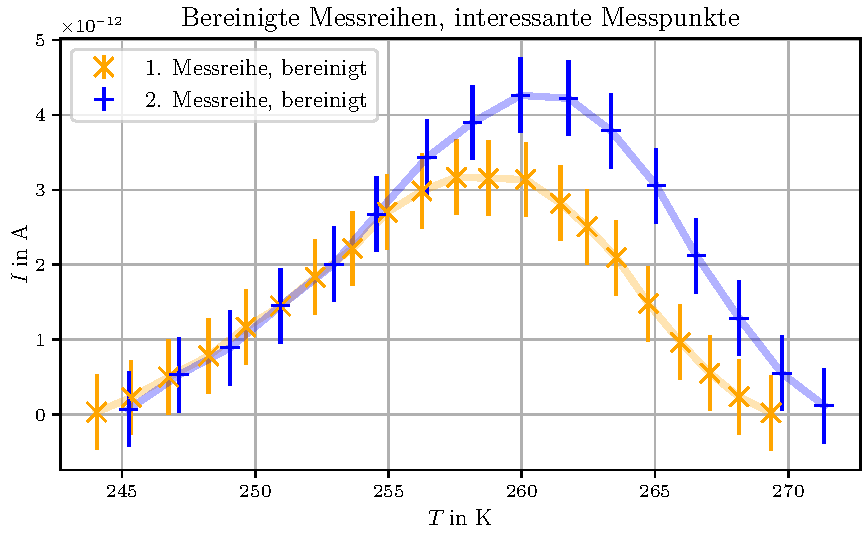
\includegraphics[width=\textwidth]{plots/F_messreihen_bereinigt_relevantepunkte.pdf}
    \caption{Die relevanten Punkte der bereinigten Daten .}
    \label{fig:Vergleich}
\end{figure}

\subsection{Berechnung über den Polarisationsansatz}
Der Logarithmus des gemessenen Stroms wird geplottet, und die Daten im kleinen Temperaturbereich werden
durch eine lineare Funktion angenähert. Die entsprechenden Ausgleichsgeraden sind in Abbildung \ref{fig:Polarisationsansatz} dargestellt.

\begin{figure}[H]
    \centering
    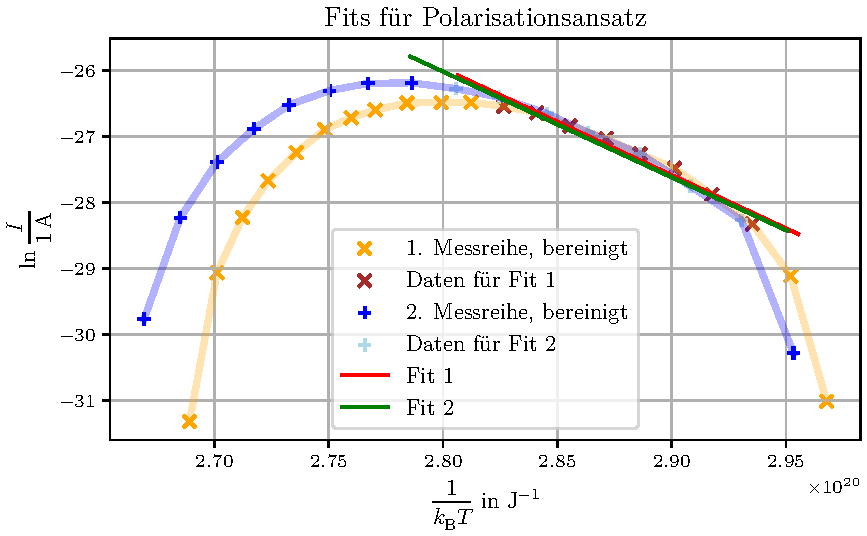
\includegraphics[width=\textwidth]{plots/G_polarisationsansatz.pdf}
    \caption{Plot von ln(I) gegen $1/k_BT$.}
    \label{fig:Polarisationsansatz}
\end{figure}

Die Aktivierungsenergie $W_i$ weird nach \ref{eq:fit_polarisationsansatz} berechnet.
Es ergeben sich für die beiden Messreihen folgende Aktivierungsenergien:
\begin{equation}
W_1 = 1.614\cdot10^{-19}\pm1.182\cdot10^{-20} J
\end{equation}
\begin{equation}
W_2 = 1.601\cdot10^{-19}\pm1.208\cdot10^{-20} J
\end{equation}

$C_i$ ist eine Konstante.
\begin{equation}
C_1 = 1.921\cdot10^1\pm3.405
\end{equation}
\begin{equation}
C_2 = 1.883\cdot10^1\pm3.463
\end{equation}
Die Relaxationszeit $\tau_i$ erhält man aus \ref{eq:tau0_maximum}
\begin{equation}
\tau_1 =  8.63\cdot10^{-20}\pm2.93\cdot10^{-19} s
\end{equation}
\begin{equation}
\tau_2 =  1.44\cdot10^{-19}\pm4.97\cdot10^{-19} s
\end{equation}

\subsection{Berechnung aus der Stromdichte}
Unter Verwendung von \ref{eq:fit_stromdichtenansatz} wird die Aktivierungsenergie über den beschriebenen Ansatz der Stromdichte 
berechnet. Es wird die Hilfsfunktion über eine einfache Summe integriert und linear interpoliert.
Es wird das Integral $I(T)$ benötigt und die Funktion 
\begin{equation}
f(T) = \ln \left( \int_{t(T)}^{\infty} I(t') \, dt' \right) - \ln I(T)
\end{equation}
berechnet die den in \ref{} Plot liefert. Einige der korrigierten Daten ergaben negative Ströme,
die aus der Analyse ausgeschlossen wurden, da sie für den untersuchten Effekt irrelevant sind.
Außerdem kann die Funktion $f(T)$ für negative Ströme nicht bestimmt werden. Die Daten werden durch eine Gerade der Form 
\begin{equation}
    f(T)=\frac{a_i}{k_BT}+b_I
\end{equation}
genähert. Bei der Regression werden nur die Datenpunkte berücksichtigt, durch die die Gerade verläuft.


\begin{figure}[H]
    \centering
    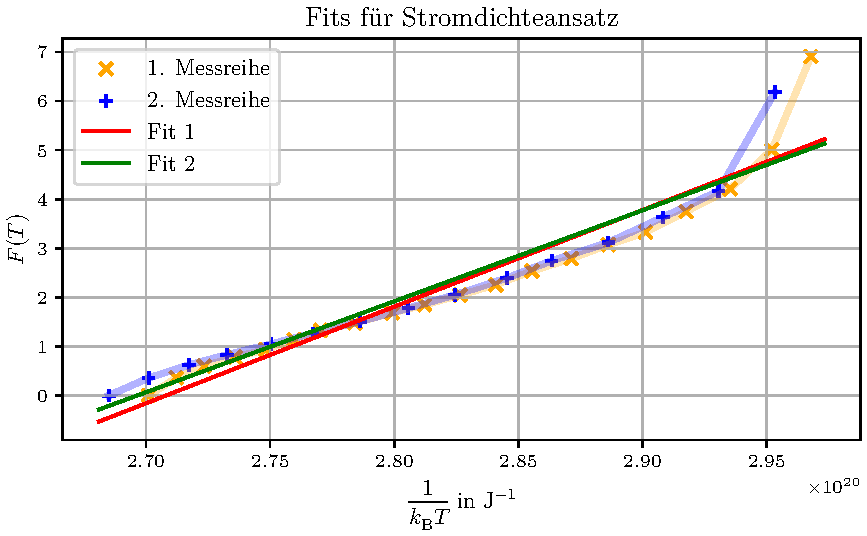
\includegraphics[width=\textwidth]{plots/H_stromdichte.pdf}
    \caption{Plot von f(T) gegen $1/k_BT$ auf logarithmischer Skala.}
    \label{fig:Stromdichteansatz}
\end{figure}

Die Aktivierungsenergie werden als 
\begin{equation}
W1   = 1.97\cdot10^{-19}\pm0.14\cdot10^{-19}J
\end{equation} 
\begin{equation}
 W2   = 1.85\cdot10^{-19}\pm0.15\cdot10^{-19}J
\end{equation} 
bestimmt.
Die Relaxationszeiten ergeben sich zu
\begin{equation}
t0_1 = 0.7\cdot10^{-23}\pm2.9\cdot10^{-23}s
\end{equation} 
\begin{equation}
t0_2 = 2\cdot10^{-22}\pm8\cdot10^{-22}s
\end{equation} 

\subsection{Relaxationszeit in Abhängigkeit der Temperatur}
Die Relaxationszeiten in Abhängigkeit von der Temperatur, basierend auf dem Polarisationsstrom,
sind in Abbildung \ref{fig:Relaxationszeit_p} dargestellt. Die entsprechenden Daten zur Stromdichte sind in Abbildung \ref{fig:Relaxationszeit_j} zu sehen.
Die Relaxationszeiten werden gemäß ihrer Formel geplottet.

\begin{figure}[H]
    \centering
    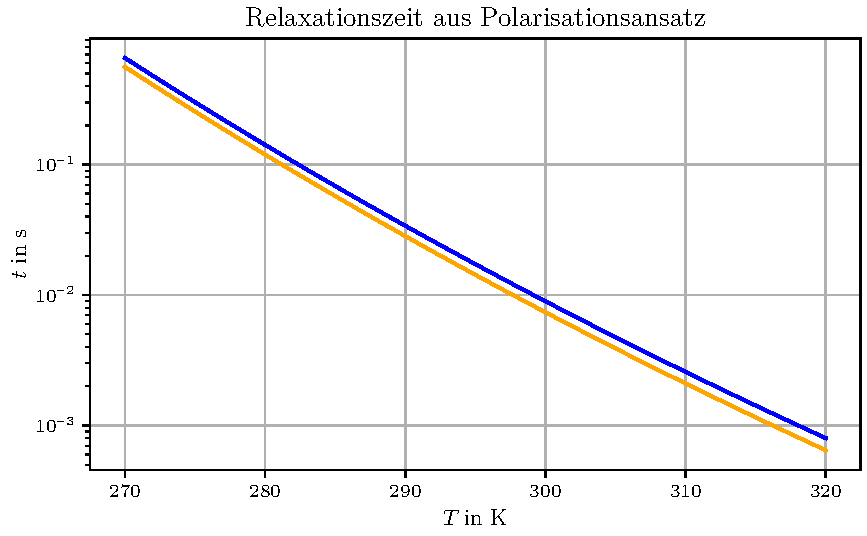
\includegraphics[width=\textwidth]{plots/I_relaxationszeit_polarisation.pdf}
    \caption{Plot der Relaxationszeit aus dem Ansatz des Polarisationsstrom in Abhängigkeit der Temperatur.
    Die erste Messreihe liefert die orangene Gerade, die zweite generiert die blaue Gerade.}
    \label{fig:Relaxationszeit_p}
\end{figure}

\begin{figure}[H]
    \centering
    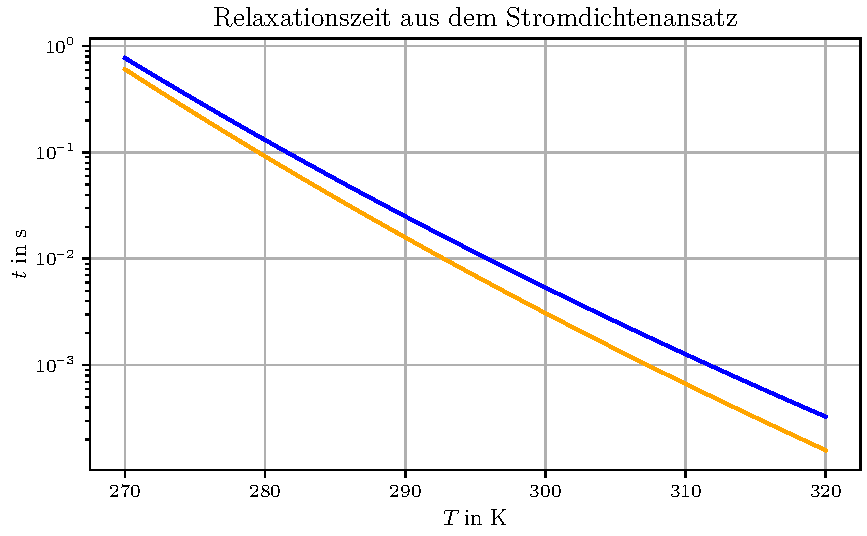
\includegraphics[width=\textwidth]{plots/J_relaxationszeit_stromdichte.pdf}
    \caption{Plot der Relaxationszeit aus dem Ansatz der Stromdichte in Abhängigkeit der Temperatur.
    Die erste Messreihe liefert die orangene Gerade, die zweite generiert die blaue Gerade.}
    \label{fig:Relaxationszeit_j}
\end{figure}